\documentclass[a4paper]{article}

\usepackage[czech]{babel} %https://github.com/michal-h21/biblatex-iso690
\usepackage[
   backend=biber      % if we want unicode 
  ,style=iso-numeric % or iso-numeric for numeric citation method          
  ,babel=other        % to support multiple languages in bibliography
  ,sortlocale=cs_CZ   % locale of main language, it is for sorting
  ,bibencoding=UTF8   % this is necessary only if bibliography file is in different encoding than main document
]{biblatex}

\usepackage[utf8]{inputenc}
\usepackage{fancyhdr}
\usepackage{amsmath}
\usepackage{amssymb}
\usepackage[left=2cm,right=2cm,top=2.5cm,bottom=2.5cm]{geometry}
\usepackage{graphicx}
\usepackage{pdfpages}
\usepackage{url}

\usepackage{siunitx}
\sisetup{locale = DE}  %, separate-uncertainty = true    kdybych chtel +/-

\usepackage{float}
\newfloat{graph}{htbp}{grp}
\floatname{graph}{Graf}
\newfloat{tabulka}{htbp}{tbl}
\floatname{tabulka}{Tabulka}

\renewcommand{\thefootnote}{\roman{footnote}}

\pagestyle{fancy}
\lhead{Praktikum IV - (A10-B) Studium relaxací NMR v roztocích (část nadstavbová)}
\rhead{Vladislav Wohlrath}
\author{Vladislav Wohlrath}

\bibliography{source}

\begin{document}

\begin{titlepage}
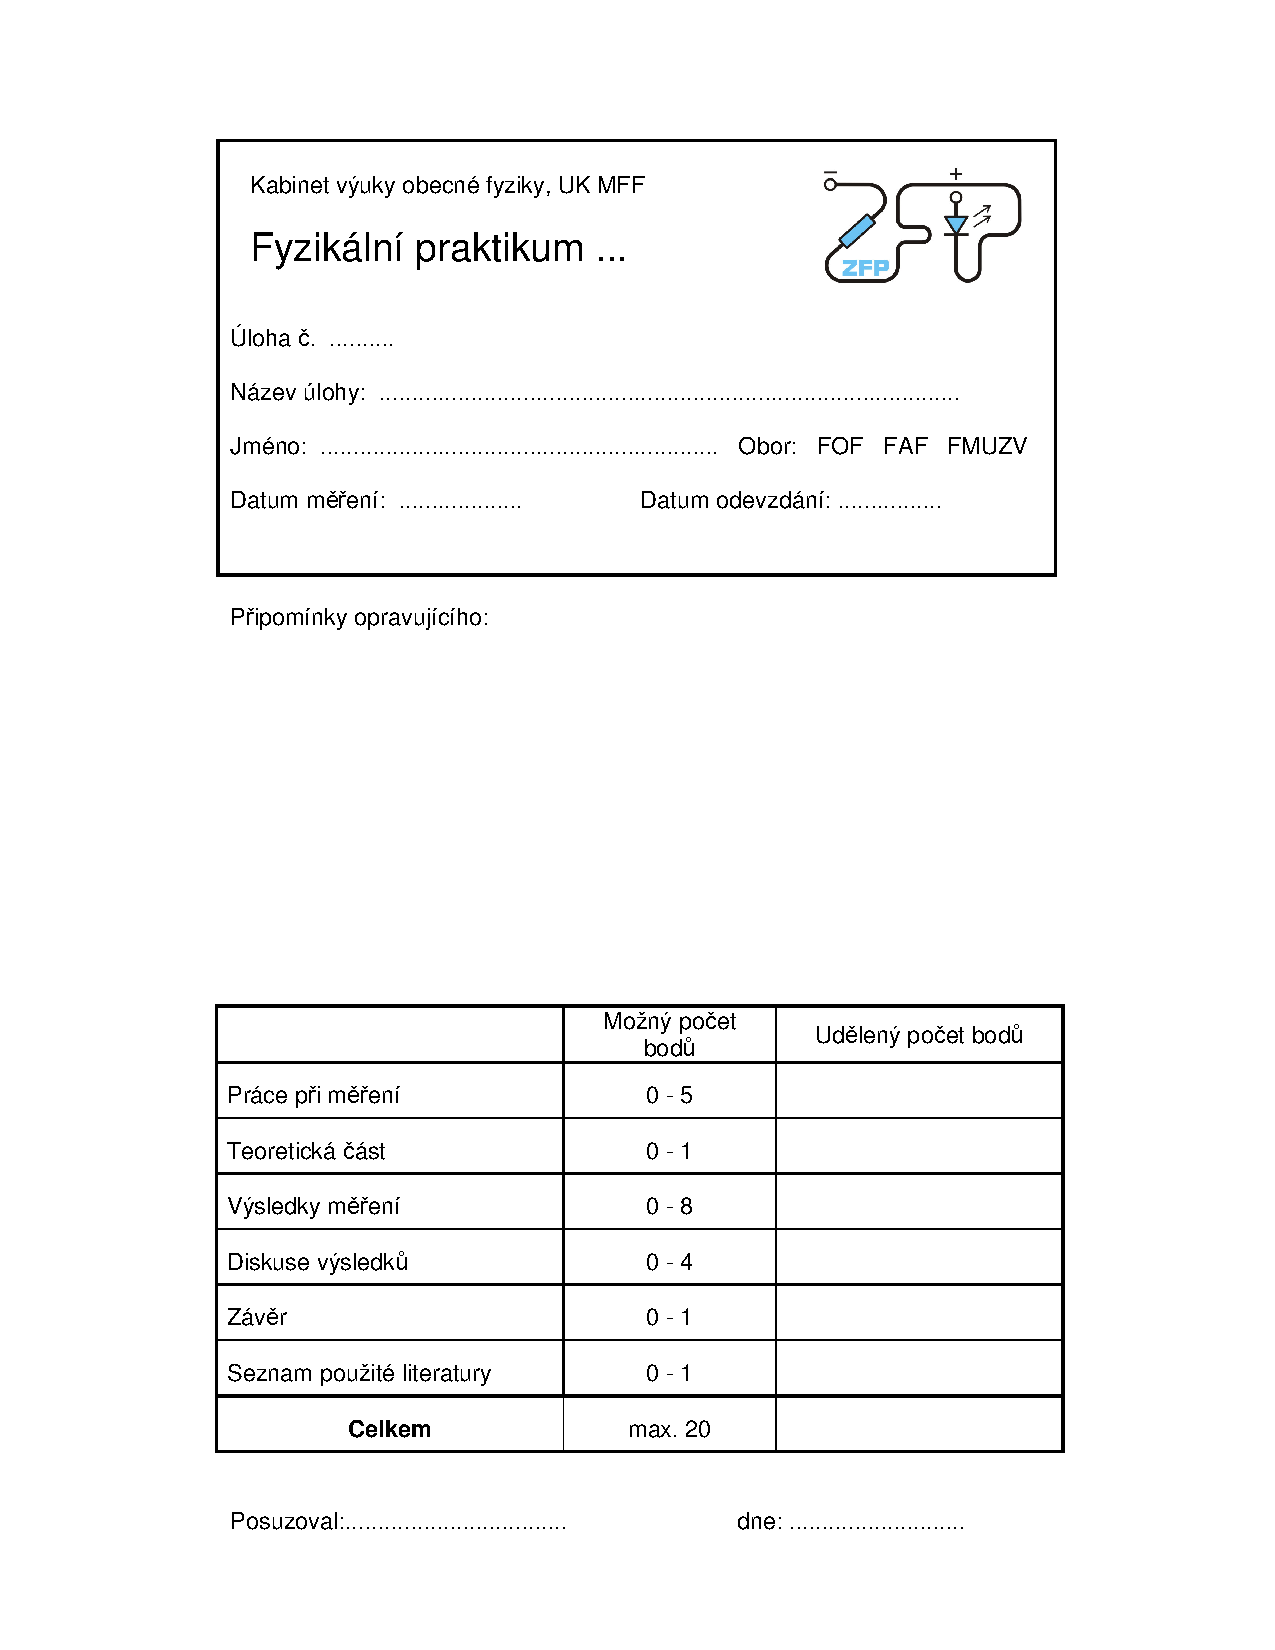
\includepdf[pages={1}]{./graficos/titlelist.pdf}
\end{titlepage}

\section*{Pracovní úkoly}
\begin{enumerate}
\item Měření spin-mřížkové relaxační doby $T_1$ signálu NMR $^1$H v roztocích s proměnnou koncentrací CuSO$_4$ metodou ($\pi$, $\pi/2$) pulsu („inversion recovery“).
\item Měření spin-spinové relaxační doby $T_2$ signálu NMR $^1$H v roztocích s proměnnou koncentrací CuSO$_4$ metodou spinového echa.
\end{enumerate}

%Teoretická část
\section*{Teoretická část}
Při metodě "inversion recovery" (IR) použijeme $\pi$-pulz ke změně znaménka podélné složky magnetizace. 
Tu pak necháme relaxovat a po čase $t_w$ použijeme $\pi/2$ pulz k otočení magnetizace do příčného směru.
Poté budeme pozorovat FID signál, jehož amplituda bude \cite{skripta}
\begin{equation} \label{e:IR}
A_{FID}(t_w)= A_0 | 1 - 2 \exp(-t_w/T_1)  | \,,
\end{equation}
kde $A_0$ je konstanta a $T_1$ je spin-mřížková relaxační doba.

Spin-spinovou relaxační dobu $T_2$ změříme podle závislosti amplitudy signálu spinového echa (SE) na odstupu pulzů $t_w$, která má podle \cite{skripta} tvar
\begin{equation} \label{e:SE}
A_{SE}(t_w)=A_1 \exp(-2t_w/T_1) \exp(-kt_w^3) \,,
\end{equation}
kde $A_1$ a $k$ jsou konstanty.

U málo viskózních kapalin platí přibližně \cite{skripta}
\begin{equation}
T_1 \approxeq T_2 \,.
\end{equation}

Paramagnetické příměsy v diamagnetických kapalinách výrazně zkracují obě relaxační doby $T_1$ i $T_2$ \cite{skripta}. Podle \cite{skripta} platí, že relaxační rychlost je přímo úměrná molární objemové koncentraci iontů Cu$^{2+}$
\begin{equation} \label{e:C}
\frac{1}{T_1} \propto c_{\text{Cu}^{2+}} \,.
\end{equation}

%Výsledky měření
\section*{Výsledky měření}
Teplota v laboratoři byla přibližně \SI{20}{\degreeCelsius}.

Měřili jsme 5 vzorků s různou koncentrací CuSO$_4$.
Naměřené závislosti jsme nafitovali závislostmi \eqref{e:IR} a \eqref{e:SE} (viz graf \ref{g:g}). 
Z těchto závislostí jsme určili relaxační doby $T_1$ a $T_2$ (viz tabulka \ref{t:T} a graf \ref{g:T}).
Relaxační rychlosti (převrácené hodnoty relaxačních dob) jsme zanesli do grafu \ref{g:rT} a nafitovali lineární a afinní funkcí pro spin-mřížkovou respektive spin-spinovou relaxační rychlost (viz \emph{Diskuze})\footnote{zápis $c_{\text{CuSO}_4}(\si{\milli M})$ znamená molární objemovou koncentraci vyjádřenou v jednotkách \si{\milli M} }
\begin{equation*}
T_1 \approx \frac{\SI{974}{\milli\second}}{c_{\text{CuSO}_4}(\si{\milli M})}
\end{equation*}
\begin{equation*}
T_2 \approx \frac{\SI{756}{\milli\second}}{c_{\text{CuSO}_4}(\si{\milli M})  - 5,08}
\end{equation*}


\begin{graph}[htbp] 
\centering
% GNUPLOT: LaTeX picture with Postscript
\begingroup
  \makeatletter
  \providecommand\color[2][]{%
    \GenericError{(gnuplot) \space\space\space\@spaces}{%
      Package color not loaded in conjunction with
      terminal option `colourtext'%
    }{See the gnuplot documentation for explanation.%
    }{Either use 'blacktext' in gnuplot or load the package
      color.sty in LaTeX.}%
    \renewcommand\color[2][]{}%
  }%
  \providecommand\includegraphics[2][]{%
    \GenericError{(gnuplot) \space\space\space\@spaces}{%
      Package graphicx or graphics not loaded%
    }{See the gnuplot documentation for explanation.%
    }{The gnuplot epslatex terminal needs graphicx.sty or graphics.sty.}%
    \renewcommand\includegraphics[2][]{}%
  }%
  \providecommand\rotatebox[2]{#2}%
  \@ifundefined{ifGPcolor}{%
    \newif\ifGPcolor
    \GPcolorfalse
  }{}%
  \@ifundefined{ifGPblacktext}{%
    \newif\ifGPblacktext
    \GPblacktexttrue
  }{}%
  % define a \g@addto@macro without @ in the name:
  \let\gplgaddtomacro\g@addto@macro
  % define empty templates for all commands taking text:
  \gdef\gplbacktext{}%
  \gdef\gplfronttext{}%
  \makeatother
  \ifGPblacktext
    % no textcolor at all
    \def\colorrgb#1{}%
    \def\colorgray#1{}%
  \else
    % gray or color?
    \ifGPcolor
      \def\colorrgb#1{\color[rgb]{#1}}%
      \def\colorgray#1{\color[gray]{#1}}%
      \expandafter\def\csname LTw\endcsname{\color{white}}%
      \expandafter\def\csname LTb\endcsname{\color{black}}%
      \expandafter\def\csname LTa\endcsname{\color{black}}%
      \expandafter\def\csname LT0\endcsname{\color[rgb]{1,0,0}}%
      \expandafter\def\csname LT1\endcsname{\color[rgb]{0,1,0}}%
      \expandafter\def\csname LT2\endcsname{\color[rgb]{0,0,1}}%
      \expandafter\def\csname LT3\endcsname{\color[rgb]{1,0,1}}%
      \expandafter\def\csname LT4\endcsname{\color[rgb]{0,1,1}}%
      \expandafter\def\csname LT5\endcsname{\color[rgb]{1,1,0}}%
      \expandafter\def\csname LT6\endcsname{\color[rgb]{0,0,0}}%
      \expandafter\def\csname LT7\endcsname{\color[rgb]{1,0.3,0}}%
      \expandafter\def\csname LT8\endcsname{\color[rgb]{0.5,0.5,0.5}}%
    \else
      % gray
      \def\colorrgb#1{\color{black}}%
      \def\colorgray#1{\color[gray]{#1}}%
      \expandafter\def\csname LTw\endcsname{\color{white}}%
      \expandafter\def\csname LTb\endcsname{\color{black}}%
      \expandafter\def\csname LTa\endcsname{\color{black}}%
      \expandafter\def\csname LT0\endcsname{\color{black}}%
      \expandafter\def\csname LT1\endcsname{\color{black}}%
      \expandafter\def\csname LT2\endcsname{\color{black}}%
      \expandafter\def\csname LT3\endcsname{\color{black}}%
      \expandafter\def\csname LT4\endcsname{\color{black}}%
      \expandafter\def\csname LT5\endcsname{\color{black}}%
      \expandafter\def\csname LT6\endcsname{\color{black}}%
      \expandafter\def\csname LT7\endcsname{\color{black}}%
      \expandafter\def\csname LT8\endcsname{\color{black}}%
    \fi
  \fi
  \setlength{\unitlength}{0.0500bp}%
  \begin{picture}(10204.00,13606.00)%
    \gplgaddtomacro\gplbacktext{%
      \csname LTb\endcsname%
      \put(330,11104){\makebox(0,0){\strut{} 0}}%
      \csname LTb\endcsname%
      \put(1140,11104){\makebox(0,0){\strut{} 50}}%
      \csname LTb\endcsname%
      \put(1950,11104){\makebox(0,0){\strut{} 100}}%
      \csname LTb\endcsname%
      \put(2761,11104){\makebox(0,0){\strut{} 150}}%
      \csname LTb\endcsname%
      \put(3571,11104){\makebox(0,0){\strut{} 200}}%
      \csname LTb\endcsname%
      \put(4381,11104){\makebox(0,0){\strut{} 250}}%
    }%
    \gplgaddtomacro\gplfronttext{%
      \csname LTb\endcsname%
      \put(3718,11497){\makebox(0,0)[r]{\strut{}IR, č. 1}}%
    }%
    \gplgaddtomacro\gplbacktext{%
      \csname LTb\endcsname%
      \put(5432,11104){\makebox(0,0){\strut{} 0}}%
      \csname LTb\endcsname%
      \put(6105,11104){\makebox(0,0){\strut{} 20}}%
      \csname LTb\endcsname%
      \put(6778,11104){\makebox(0,0){\strut{} 40}}%
      \csname LTb\endcsname%
      \put(7451,11104){\makebox(0,0){\strut{} 60}}%
      \csname LTb\endcsname%
      \put(8124,11104){\makebox(0,0){\strut{} 80}}%
      \csname LTb\endcsname%
      \put(8797,11104){\makebox(0,0){\strut{} 100}}%
      \csname LTb\endcsname%
      \put(9470,11104){\makebox(0,0){\strut{} 120}}%
    }%
    \gplgaddtomacro\gplfronttext{%
      \csname LTb\endcsname%
      \put(8820,11497){\makebox(0,0)[r]{\strut{}IR, č. 2}}%
    }%
    \gplgaddtomacro\gplbacktext{%
      \csname LTb\endcsname%
      \put(330,8383){\makebox(0,0){\strut{} 0}}%
      \csname LTb\endcsname%
      \put(1125,8383){\makebox(0,0){\strut{} 20}}%
      \csname LTb\endcsname%
      \put(1921,8383){\makebox(0,0){\strut{} 40}}%
      \csname LTb\endcsname%
      \put(2716,8383){\makebox(0,0){\strut{} 60}}%
      \csname LTb\endcsname%
      \put(3512,8383){\makebox(0,0){\strut{} 80}}%
      \csname LTb\endcsname%
      \put(4307,8383){\makebox(0,0){\strut{} 100}}%
    }%
    \gplgaddtomacro\gplfronttext{%
      \csname LTb\endcsname%
      \put(3718,8776){\makebox(0,0)[r]{\strut{}IR, č. 3}}%
    }%
    \gplgaddtomacro\gplbacktext{%
      \csname LTb\endcsname%
      \put(5432,8383){\makebox(0,0){\strut{} 0}}%
      \csname LTb\endcsname%
      \put(6227,8383){\makebox(0,0){\strut{} 20}}%
      \csname LTb\endcsname%
      \put(7023,8383){\makebox(0,0){\strut{} 40}}%
      \csname LTb\endcsname%
      \put(7818,8383){\makebox(0,0){\strut{} 60}}%
      \csname LTb\endcsname%
      \put(8614,8383){\makebox(0,0){\strut{} 80}}%
      \csname LTb\endcsname%
      \put(9409,8383){\makebox(0,0){\strut{} 100}}%
    }%
    \gplgaddtomacro\gplfronttext{%
      \csname LTb\endcsname%
      \put(8820,8776){\makebox(0,0)[r]{\strut{}IR, č. 4}}%
    }%
    \gplgaddtomacro\gplbacktext{%
      \csname LTb\endcsname%
      \put(330,5662){\makebox(0,0){\strut{} 0}}%
      \csname LTb\endcsname%
      \put(816,5662){\makebox(0,0){\strut{} 10}}%
      \csname LTb\endcsname%
      \put(1302,5662){\makebox(0,0){\strut{} 20}}%
      \csname LTb\endcsname%
      \put(1788,5662){\makebox(0,0){\strut{} 30}}%
      \csname LTb\endcsname%
      \put(2274,5662){\makebox(0,0){\strut{} 40}}%
      \csname LTb\endcsname%
      \put(2761,5662){\makebox(0,0){\strut{} 50}}%
      \csname LTb\endcsname%
      \put(3247,5662){\makebox(0,0){\strut{} 60}}%
      \csname LTb\endcsname%
      \put(3733,5662){\makebox(0,0){\strut{} 70}}%
      \csname LTb\endcsname%
      \put(4219,5662){\makebox(0,0){\strut{} 80}}%
      \csname LTb\endcsname%
      \put(4705,5662){\makebox(0,0){\strut{} 90}}%
    }%
    \gplgaddtomacro\gplfronttext{%
      \csname LTb\endcsname%
      \put(3718,6055){\makebox(0,0)[r]{\strut{}IR, č. 5}}%
    }%
    \gplgaddtomacro\gplbacktext{%
      \csname LTb\endcsname%
      \put(5432,5662){\makebox(0,0){\strut{} 0}}%
      \csname LTb\endcsname%
      \put(5918,5662){\makebox(0,0){\strut{} 5}}%
      \csname LTb\endcsname%
      \put(6404,5662){\makebox(0,0){\strut{} 10}}%
      \csname LTb\endcsname%
      \put(6890,5662){\makebox(0,0){\strut{} 15}}%
      \csname LTb\endcsname%
      \put(7376,5662){\makebox(0,0){\strut{} 20}}%
      \csname LTb\endcsname%
      \put(7863,5662){\makebox(0,0){\strut{} 25}}%
      \csname LTb\endcsname%
      \put(8349,5662){\makebox(0,0){\strut{} 30}}%
      \csname LTb\endcsname%
      \put(8835,5662){\makebox(0,0){\strut{} 35}}%
      \csname LTb\endcsname%
      \put(9321,5662){\makebox(0,0){\strut{} 40}}%
      \csname LTb\endcsname%
      \put(9807,5662){\makebox(0,0){\strut{} 45}}%
    }%
    \gplgaddtomacro\gplfronttext{%
      \csname LTb\endcsname%
      \put(8820,7726){\makebox(0,0)[r]{\strut{}SE, č. 1}}%
    }%
    \gplgaddtomacro\gplbacktext{%
      \csname LTb\endcsname%
      \put(330,2941){\makebox(0,0){\strut{} 0}}%
      \csname LTb\endcsname%
      \put(877,2941){\makebox(0,0){\strut{} 5}}%
      \csname LTb\endcsname%
      \put(1424,2941){\makebox(0,0){\strut{} 10}}%
      \csname LTb\endcsname%
      \put(1971,2941){\makebox(0,0){\strut{} 15}}%
      \csname LTb\endcsname%
      \put(2518,2941){\makebox(0,0){\strut{} 20}}%
      \csname LTb\endcsname%
      \put(3064,2941){\makebox(0,0){\strut{} 25}}%
      \csname LTb\endcsname%
      \put(3611,2941){\makebox(0,0){\strut{} 30}}%
      \csname LTb\endcsname%
      \put(4158,2941){\makebox(0,0){\strut{} 35}}%
      \csname LTb\endcsname%
      \put(4705,2941){\makebox(0,0){\strut{} 40}}%
    }%
    \gplgaddtomacro\gplfronttext{%
      \csname LTb\endcsname%
      \put(3718,5005){\makebox(0,0)[r]{\strut{}SE, č. 2}}%
    }%
    \gplgaddtomacro\gplbacktext{%
      \csname LTb\endcsname%
      \put(5432,2941){\makebox(0,0){\strut{} 0}}%
      \csname LTb\endcsname%
      \put(5979,2941){\makebox(0,0){\strut{} 5}}%
      \csname LTb\endcsname%
      \put(6526,2941){\makebox(0,0){\strut{} 10}}%
      \csname LTb\endcsname%
      \put(7073,2941){\makebox(0,0){\strut{} 15}}%
      \csname LTb\endcsname%
      \put(7620,2941){\makebox(0,0){\strut{} 20}}%
      \csname LTb\endcsname%
      \put(8166,2941){\makebox(0,0){\strut{} 25}}%
      \csname LTb\endcsname%
      \put(8713,2941){\makebox(0,0){\strut{} 30}}%
      \csname LTb\endcsname%
      \put(9260,2941){\makebox(0,0){\strut{} 35}}%
      \csname LTb\endcsname%
      \put(9807,2941){\makebox(0,0){\strut{} 40}}%
    }%
    \gplgaddtomacro\gplfronttext{%
      \csname LTb\endcsname%
      \put(8820,5005){\makebox(0,0)[r]{\strut{}SE, č. 3}}%
    }%
    \gplgaddtomacro\gplbacktext{%
      \csname LTb\endcsname%
      \put(330,220){\makebox(0,0){\strut{} 0}}%
      \csname LTb\endcsname%
      \put(955,220){\makebox(0,0){\strut{} 5}}%
      \csname LTb\endcsname%
      \put(1580,220){\makebox(0,0){\strut{} 10}}%
      \csname LTb\endcsname%
      \put(2205,220){\makebox(0,0){\strut{} 15}}%
      \csname LTb\endcsname%
      \put(2830,220){\makebox(0,0){\strut{} 20}}%
      \csname LTb\endcsname%
      \put(3455,220){\makebox(0,0){\strut{} 25}}%
      \csname LTb\endcsname%
      \put(4080,220){\makebox(0,0){\strut{} 30}}%
      \csname LTb\endcsname%
      \put(4705,220){\makebox(0,0){\strut{} 35}}%
    }%
    \gplgaddtomacro\gplfronttext{%
      \csname LTb\endcsname%
      \put(3718,2284){\makebox(0,0)[r]{\strut{}SE, č. 4}}%
    }%
    \gplgaddtomacro\gplbacktext{%
      \csname LTb\endcsname%
      \put(5432,220){\makebox(0,0){\strut{} 0}}%
      \csname LTb\endcsname%
      \put(6307,220){\makebox(0,0){\strut{} 5}}%
      \csname LTb\endcsname%
      \put(7182,220){\makebox(0,0){\strut{} 10}}%
      \csname LTb\endcsname%
      \put(8057,220){\makebox(0,0){\strut{} 15}}%
      \csname LTb\endcsname%
      \put(8932,220){\makebox(0,0){\strut{} 20}}%
      \csname LTb\endcsname%
      \put(9807,220){\makebox(0,0){\strut{} 25}}%
    }%
    \gplgaddtomacro\gplfronttext{%
      \csname LTb\endcsname%
      \put(8820,2284){\makebox(0,0)[r]{\strut{}SE, č. 5}}%
    }%
    \gplbacktext
    \put(0,0){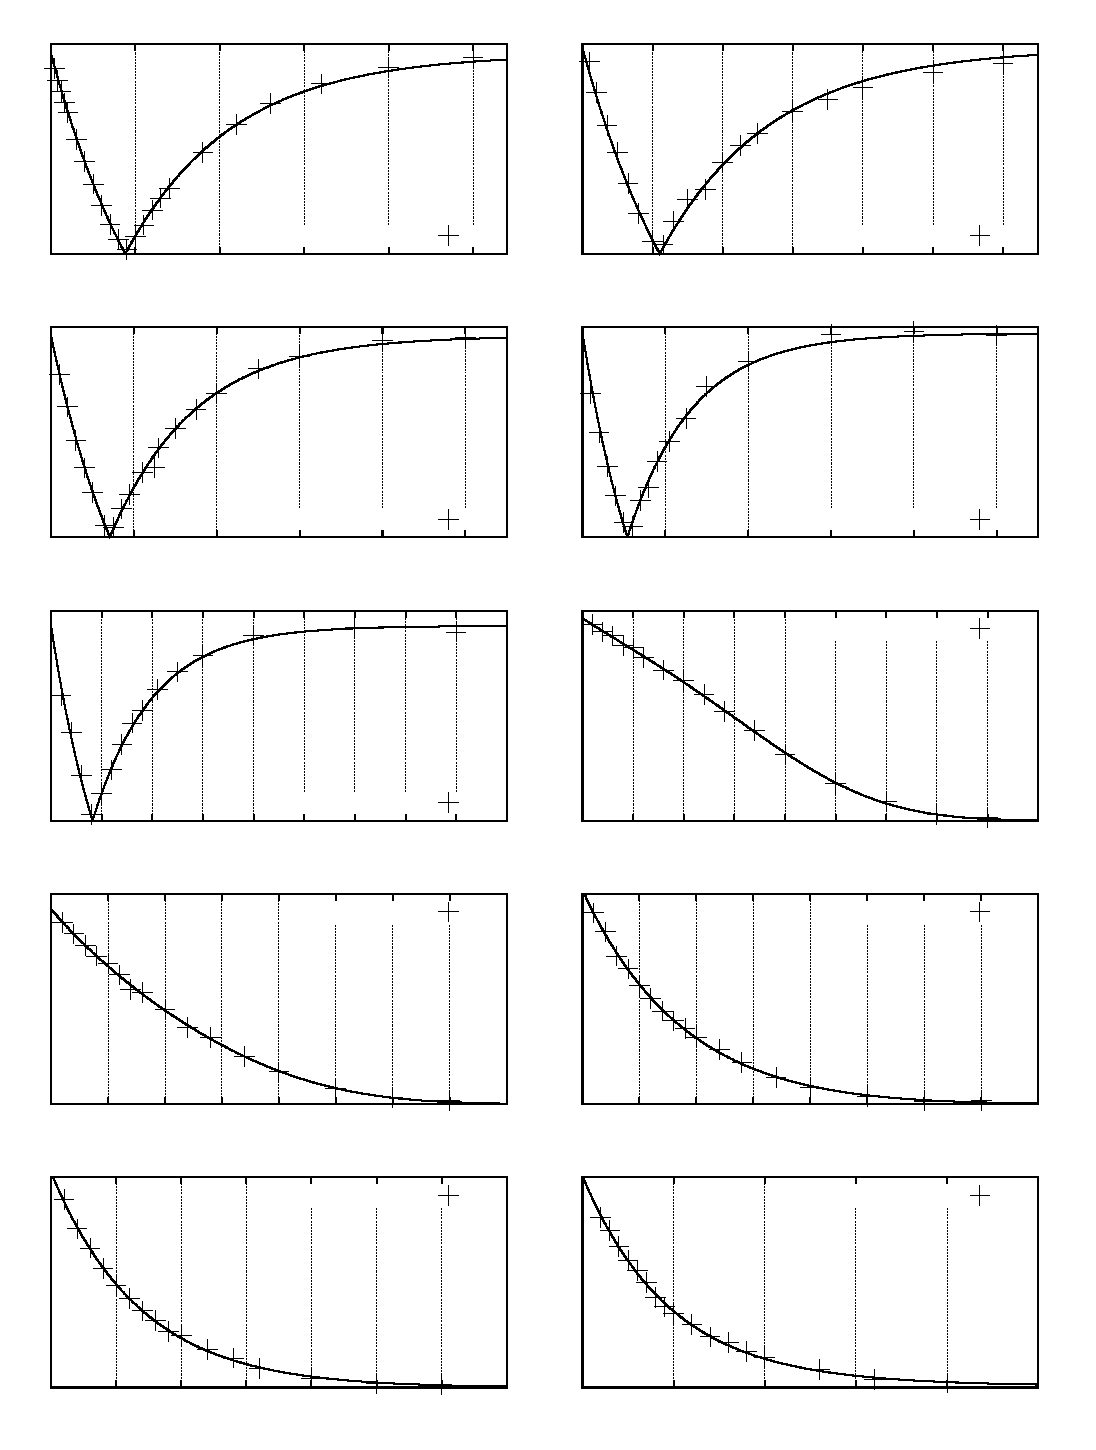
\includegraphics{g}}%
    \gplfronttext
  \end{picture}%
\endgroup

\caption{Závislost amplitudy signálu na odstupu pulzů $t_w$ (osa $x$ (\si{\ms})).}
\label{g:g}
\end{graph}

\begin{tabulka}[htbp]
\centering
\begin{tabular}{c|ccc}
číslo vzorku & $c_{\text{CuSO}_4}$ (\si{\milli M}) & $T_1$ (\si{\ms}) & $T_2$ (\si{\ms}) \\
\hline
1 & 16 & \num{63.5(3)} & \num{61.6(20)} \\
2 & 32 & \num{31.8(4)} & \num{29.4(8)} \\
3 & 48 & \num{20.5(2)} & \num{17.3(4)} \\
4 & 64 & \num{15.6(3)} & \num{13.6(3)} \\
5 & 80 & \num{11.8(2)} & \num{9.8(3)} \\
\end{tabular}
\caption{Relaxační doby signálu NMR $^1$H v roztocích s proměnnou koncentrací CuSO$_4$}
\label{t:T}
\end{tabulka}

\begin{graph}[htbp] 
\centering
% GNUPLOT: LaTeX picture with Postscript
\begingroup
  \makeatletter
  \providecommand\color[2][]{%
    \GenericError{(gnuplot) \space\space\space\@spaces}{%
      Package color not loaded in conjunction with
      terminal option `colourtext'%
    }{See the gnuplot documentation for explanation.%
    }{Either use 'blacktext' in gnuplot or load the package
      color.sty in LaTeX.}%
    \renewcommand\color[2][]{}%
  }%
  \providecommand\includegraphics[2][]{%
    \GenericError{(gnuplot) \space\space\space\@spaces}{%
      Package graphicx or graphics not loaded%
    }{See the gnuplot documentation for explanation.%
    }{The gnuplot epslatex terminal needs graphicx.sty or graphics.sty.}%
    \renewcommand\includegraphics[2][]{}%
  }%
  \providecommand\rotatebox[2]{#2}%
  \@ifundefined{ifGPcolor}{%
    \newif\ifGPcolor
    \GPcolorfalse
  }{}%
  \@ifundefined{ifGPblacktext}{%
    \newif\ifGPblacktext
    \GPblacktexttrue
  }{}%
  % define a \g@addto@macro without @ in the name:
  \let\gplgaddtomacro\g@addto@macro
  % define empty templates for all commands taking text:
  \gdef\gplbacktext{}%
  \gdef\gplfronttext{}%
  \makeatother
  \ifGPblacktext
    % no textcolor at all
    \def\colorrgb#1{}%
    \def\colorgray#1{}%
  \else
    % gray or color?
    \ifGPcolor
      \def\colorrgb#1{\color[rgb]{#1}}%
      \def\colorgray#1{\color[gray]{#1}}%
      \expandafter\def\csname LTw\endcsname{\color{white}}%
      \expandafter\def\csname LTb\endcsname{\color{black}}%
      \expandafter\def\csname LTa\endcsname{\color{black}}%
      \expandafter\def\csname LT0\endcsname{\color[rgb]{1,0,0}}%
      \expandafter\def\csname LT1\endcsname{\color[rgb]{0,1,0}}%
      \expandafter\def\csname LT2\endcsname{\color[rgb]{0,0,1}}%
      \expandafter\def\csname LT3\endcsname{\color[rgb]{1,0,1}}%
      \expandafter\def\csname LT4\endcsname{\color[rgb]{0,1,1}}%
      \expandafter\def\csname LT5\endcsname{\color[rgb]{1,1,0}}%
      \expandafter\def\csname LT6\endcsname{\color[rgb]{0,0,0}}%
      \expandafter\def\csname LT7\endcsname{\color[rgb]{1,0.3,0}}%
      \expandafter\def\csname LT8\endcsname{\color[rgb]{0.5,0.5,0.5}}%
    \else
      % gray
      \def\colorrgb#1{\color{black}}%
      \def\colorgray#1{\color[gray]{#1}}%
      \expandafter\def\csname LTw\endcsname{\color{white}}%
      \expandafter\def\csname LTb\endcsname{\color{black}}%
      \expandafter\def\csname LTa\endcsname{\color{black}}%
      \expandafter\def\csname LT0\endcsname{\color{black}}%
      \expandafter\def\csname LT1\endcsname{\color{black}}%
      \expandafter\def\csname LT2\endcsname{\color{black}}%
      \expandafter\def\csname LT3\endcsname{\color{black}}%
      \expandafter\def\csname LT4\endcsname{\color{black}}%
      \expandafter\def\csname LT5\endcsname{\color{black}}%
      \expandafter\def\csname LT6\endcsname{\color{black}}%
      \expandafter\def\csname LT7\endcsname{\color{black}}%
      \expandafter\def\csname LT8\endcsname{\color{black}}%
    \fi
  \fi
  \setlength{\unitlength}{0.0500bp}%
  \begin{picture}(10204.00,6802.00)%
    \gplgaddtomacro\gplbacktext{%
      \csname LTb\endcsname%
      \put(1078,704){\makebox(0,0)[r]{\strut{} 0}}%
      \csname LTb\endcsname%
      \put(1078,1765){\makebox(0,0)[r]{\strut{} 0.02}}%
      \csname LTb\endcsname%
      \put(1078,2825){\makebox(0,0)[r]{\strut{} 0.04}}%
      \csname LTb\endcsname%
      \put(1078,3886){\makebox(0,0)[r]{\strut{} 0.06}}%
      \csname LTb\endcsname%
      \put(1078,4946){\makebox(0,0)[r]{\strut{} 0.08}}%
      \csname LTb\endcsname%
      \put(1078,6007){\makebox(0,0)[r]{\strut{} 0.1}}%
      \csname LTb\endcsname%
      \put(1210,484){\makebox(0,0){\strut{} 0}}%
      \csname LTb\endcsname%
      \put(2165,484){\makebox(0,0){\strut{} 10}}%
      \csname LTb\endcsname%
      \put(3120,484){\makebox(0,0){\strut{} 20}}%
      \csname LTb\endcsname%
      \put(4076,484){\makebox(0,0){\strut{} 30}}%
      \csname LTb\endcsname%
      \put(5031,484){\makebox(0,0){\strut{} 40}}%
      \csname LTb\endcsname%
      \put(5986,484){\makebox(0,0){\strut{} 50}}%
      \csname LTb\endcsname%
      \put(6941,484){\makebox(0,0){\strut{} 60}}%
      \csname LTb\endcsname%
      \put(7897,484){\makebox(0,0){\strut{} 70}}%
      \csname LTb\endcsname%
      \put(8852,484){\makebox(0,0){\strut{} 80}}%
      \csname LTb\endcsname%
      \put(9807,484){\makebox(0,0){\strut{} 90}}%
      \put(176,3620){\rotatebox{-270}{\makebox(0,0){\strut{}(\si{\per\ms})}}}%
      \put(5508,154){\makebox(0,0){\strut{}$c$ (\si{\milli M})}}%
    }%
    \gplgaddtomacro\gplfronttext{%
      \csname LTb\endcsname%
      \put(3850,6364){\makebox(0,0)[r]{\strut{}$1/T_1$}}%
      \csname LTb\endcsname%
      \put(3850,6144){\makebox(0,0)[r]{\strut{}lineární fit $1/T_1$}}%
      \csname LTb\endcsname%
      \put(3850,5924){\makebox(0,0)[r]{\strut{}$1/T_2$}}%
      \csname LTb\endcsname%
      \put(3850,5704){\makebox(0,0)[r]{\strut{}afinní fit $1/T_2$}}%
    }%
    \gplbacktext
    \put(0,0){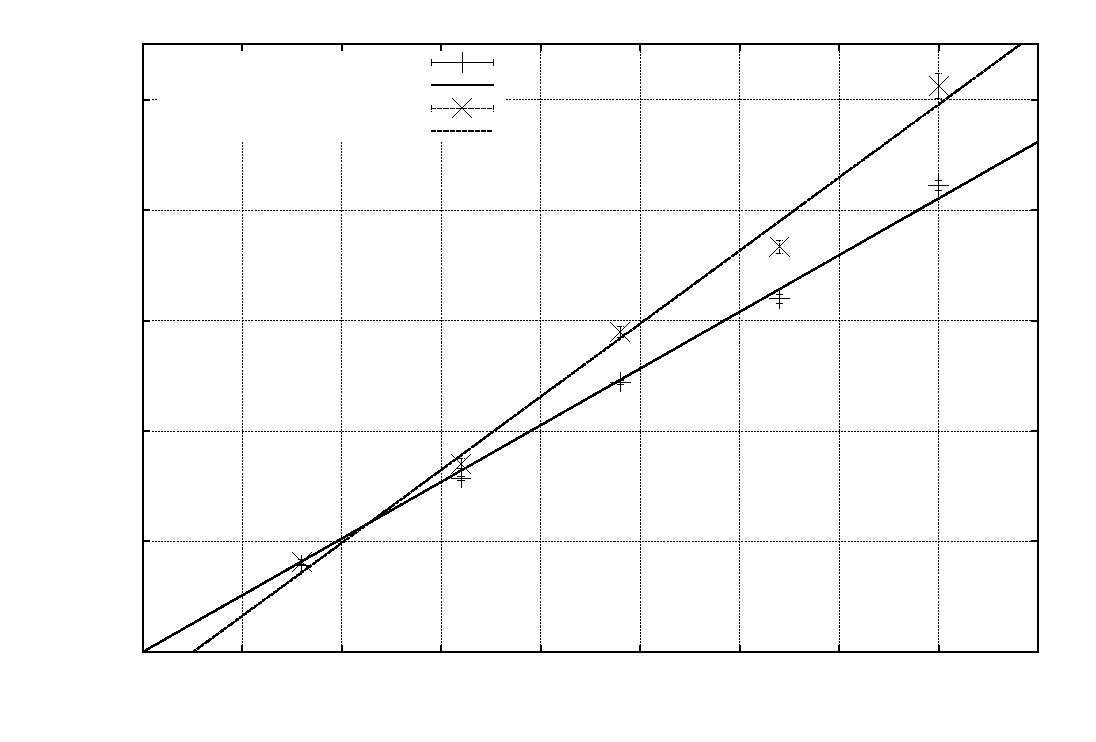
\includegraphics{rT}}%
    \gplfronttext
  \end{picture}%
\endgroup

\caption{Převrácené relaxační doby signálu NMR $^1$H v roztocích s proměnnou koncentrací CuSO$_4$}
\label{g:rT}
\end{graph}

\begin{graph}[htb] 
\centering
% GNUPLOT: LaTeX picture with Postscript
\begingroup
  \makeatletter
  \providecommand\color[2][]{%
    \GenericError{(gnuplot) \space\space\space\@spaces}{%
      Package color not loaded in conjunction with
      terminal option `colourtext'%
    }{See the gnuplot documentation for explanation.%
    }{Either use 'blacktext' in gnuplot or load the package
      color.sty in LaTeX.}%
    \renewcommand\color[2][]{}%
  }%
  \providecommand\includegraphics[2][]{%
    \GenericError{(gnuplot) \space\space\space\@spaces}{%
      Package graphicx or graphics not loaded%
    }{See the gnuplot documentation for explanation.%
    }{The gnuplot epslatex terminal needs graphicx.sty or graphics.sty.}%
    \renewcommand\includegraphics[2][]{}%
  }%
  \providecommand\rotatebox[2]{#2}%
  \@ifundefined{ifGPcolor}{%
    \newif\ifGPcolor
    \GPcolorfalse
  }{}%
  \@ifundefined{ifGPblacktext}{%
    \newif\ifGPblacktext
    \GPblacktexttrue
  }{}%
  % define a \g@addto@macro without @ in the name:
  \let\gplgaddtomacro\g@addto@macro
  % define empty templates for all commands taking text:
  \gdef\gplbacktext{}%
  \gdef\gplfronttext{}%
  \makeatother
  \ifGPblacktext
    % no textcolor at all
    \def\colorrgb#1{}%
    \def\colorgray#1{}%
  \else
    % gray or color?
    \ifGPcolor
      \def\colorrgb#1{\color[rgb]{#1}}%
      \def\colorgray#1{\color[gray]{#1}}%
      \expandafter\def\csname LTw\endcsname{\color{white}}%
      \expandafter\def\csname LTb\endcsname{\color{black}}%
      \expandafter\def\csname LTa\endcsname{\color{black}}%
      \expandafter\def\csname LT0\endcsname{\color[rgb]{1,0,0}}%
      \expandafter\def\csname LT1\endcsname{\color[rgb]{0,1,0}}%
      \expandafter\def\csname LT2\endcsname{\color[rgb]{0,0,1}}%
      \expandafter\def\csname LT3\endcsname{\color[rgb]{1,0,1}}%
      \expandafter\def\csname LT4\endcsname{\color[rgb]{0,1,1}}%
      \expandafter\def\csname LT5\endcsname{\color[rgb]{1,1,0}}%
      \expandafter\def\csname LT6\endcsname{\color[rgb]{0,0,0}}%
      \expandafter\def\csname LT7\endcsname{\color[rgb]{1,0.3,0}}%
      \expandafter\def\csname LT8\endcsname{\color[rgb]{0.5,0.5,0.5}}%
    \else
      % gray
      \def\colorrgb#1{\color{black}}%
      \def\colorgray#1{\color[gray]{#1}}%
      \expandafter\def\csname LTw\endcsname{\color{white}}%
      \expandafter\def\csname LTb\endcsname{\color{black}}%
      \expandafter\def\csname LTa\endcsname{\color{black}}%
      \expandafter\def\csname LT0\endcsname{\color{black}}%
      \expandafter\def\csname LT1\endcsname{\color{black}}%
      \expandafter\def\csname LT2\endcsname{\color{black}}%
      \expandafter\def\csname LT3\endcsname{\color{black}}%
      \expandafter\def\csname LT4\endcsname{\color{black}}%
      \expandafter\def\csname LT5\endcsname{\color{black}}%
      \expandafter\def\csname LT6\endcsname{\color{black}}%
      \expandafter\def\csname LT7\endcsname{\color{black}}%
      \expandafter\def\csname LT8\endcsname{\color{black}}%
    \fi
  \fi
  \setlength{\unitlength}{0.0500bp}%
  \begin{picture}(10204.00,6802.00)%
    \gplgaddtomacro\gplbacktext{%
      \csname LTb\endcsname%
      \put(814,704){\makebox(0,0)[r]{\strut{} 0}}%
      \csname LTb\endcsname%
      \put(814,1537){\makebox(0,0)[r]{\strut{} 10}}%
      \csname LTb\endcsname%
      \put(814,2371){\makebox(0,0)[r]{\strut{} 20}}%
      \csname LTb\endcsname%
      \put(814,3204){\makebox(0,0)[r]{\strut{} 30}}%
      \csname LTb\endcsname%
      \put(814,4037){\makebox(0,0)[r]{\strut{} 40}}%
      \csname LTb\endcsname%
      \put(814,4870){\makebox(0,0)[r]{\strut{} 50}}%
      \csname LTb\endcsname%
      \put(814,5704){\makebox(0,0)[r]{\strut{} 60}}%
      \csname LTb\endcsname%
      \put(814,6537){\makebox(0,0)[r]{\strut{} 70}}%
      \csname LTb\endcsname%
      \put(946,484){\makebox(0,0){\strut{} 0}}%
      \csname LTb\endcsname%
      \put(1931,484){\makebox(0,0){\strut{} 10}}%
      \csname LTb\endcsname%
      \put(2915,484){\makebox(0,0){\strut{} 20}}%
      \csname LTb\endcsname%
      \put(3900,484){\makebox(0,0){\strut{} 30}}%
      \csname LTb\endcsname%
      \put(4884,484){\makebox(0,0){\strut{} 40}}%
      \csname LTb\endcsname%
      \put(5869,484){\makebox(0,0){\strut{} 50}}%
      \csname LTb\endcsname%
      \put(6853,484){\makebox(0,0){\strut{} 60}}%
      \csname LTb\endcsname%
      \put(7838,484){\makebox(0,0){\strut{} 70}}%
      \csname LTb\endcsname%
      \put(8822,484){\makebox(0,0){\strut{} 80}}%
      \csname LTb\endcsname%
      \put(9807,484){\makebox(0,0){\strut{} 90}}%
      \put(176,3620){\rotatebox{-270}{\makebox(0,0){\strut{}(\si{\ms})}}}%
      \put(5376,154){\makebox(0,0){\strut{}$c$ (\si{\milli M})}}%
    }%
    \gplgaddtomacro\gplfronttext{%
      \csname LTb\endcsname%
      \put(8820,6364){\makebox(0,0)[r]{\strut{}$T_1$}}%
      \csname LTb\endcsname%
      \put(8820,6144){\makebox(0,0)[r]{\strut{}lineární fit $1/T_1$}}%
      \csname LTb\endcsname%
      \put(8820,5924){\makebox(0,0)[r]{\strut{}$T_2$}}%
      \csname LTb\endcsname%
      \put(8820,5704){\makebox(0,0)[r]{\strut{}afinní fit $1/T_2$}}%
    }%
    \gplbacktext
    \put(0,0){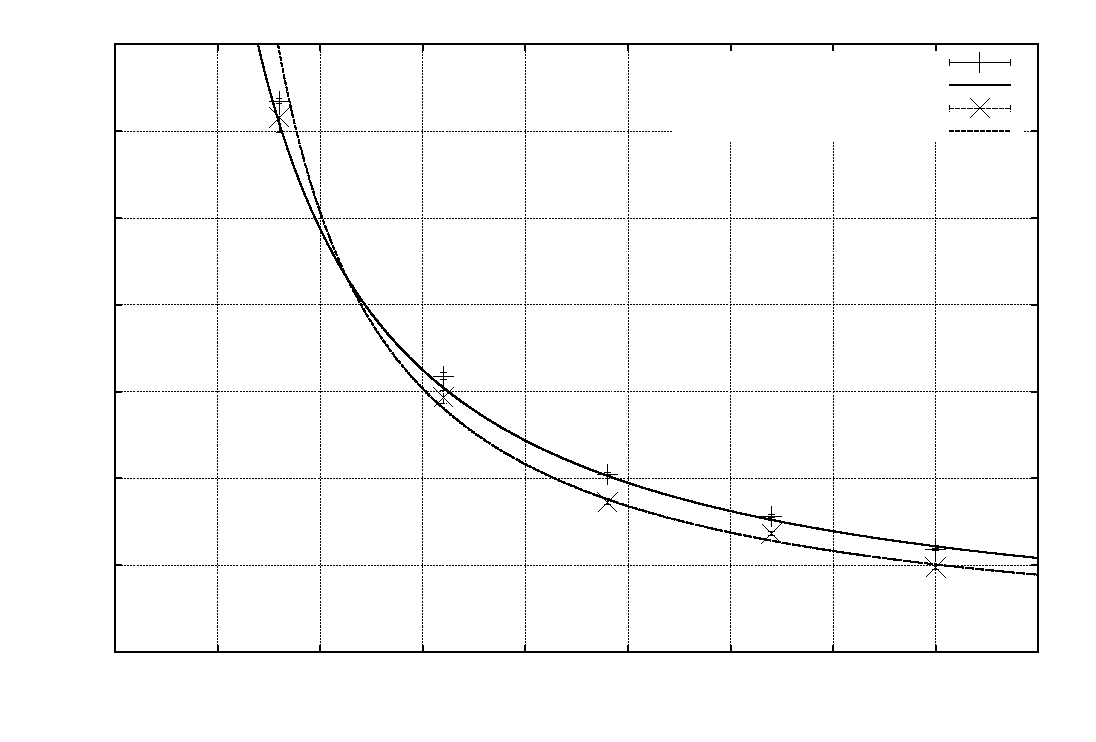
\includegraphics{T}}%
    \gplfronttext
  \end{picture}%
\endgroup

\caption{Relaxační doby signálu NMR $^1$H v roztocích s proměnnou koncentrací CuSO$_4$}
\label{g:T}
\end{graph}




%Diskuze výsledků
\section*{Diskuze}

%Závěr
\section*{Závěr}
Měřili jsme relaxační doby $T_1$ a $T_2$ signálu NMR $^1$H v roztocích s proměnnou koncentrací CuSO$_4$ metodou inversion recovery respektive spinového echa (viz tabulka \ref{t:T}).
Obě relaxační doby se pro každý vzorek přibližně rovnaly a byly nepřímo úměrné koncentraci CuSO$_4$ (viz graf \ref{g:T}).


\printbibliography[title={Seznam použité literatury}]

\end{document}